\documentclass[tikz,border=6pt]{standalone}
\usepackage{amsmath,amssymb,mathtools}
\usepackage{xcolor}
\usepackage{tikz}
\usetikzlibrary{arrows.meta,calc,positioning,decorations.pathmorphing}

\definecolor{cobalt}{HTML}{2b4c7e}
\definecolor{navyhead}{HTML}{1a365d}
\definecolor{boxblue}{HTML}{eef3fa}
\definecolor{boxgreen}{HTML}{eaf6f0}
\definecolor{ruleblue}{HTML}{2b6cb0}
\definecolor{rulegold}{HTML}{b7791f}
\definecolor{rulered}{HTML}{c0392b}
\definecolor{rulegreen}{HTML}{1f8a5f}

\begin{document}
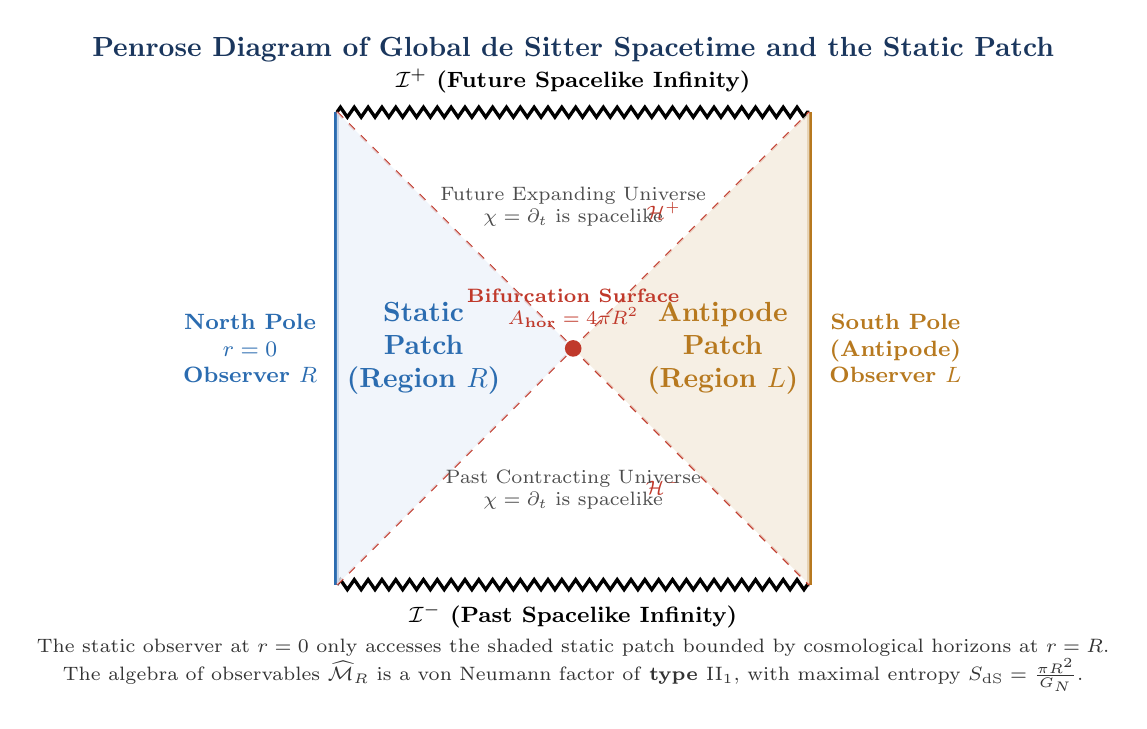
\begin{tikzpicture}[>=Latex, font=\small]

  % Title
  \node[font=\bfseries\normalsize\color{navyhead}, align=center] at (3.0, 6.8) 
    {Penrose Diagram of Global de Sitter Spacetime and the Static Patch};

  % Square de Sitter Penrose diagram
  % Corners at (0,0), (6,0), (6,6), (0,6)
  
  % Future and Past spacelike infinities (wavy double lines)
  \draw[decorate, decoration={zigzag, segment length=5pt, amplitude=1.8pt}, line width=1.2pt] 
    (0, 6.0) -- (6.0, 6.0) node[midway, above=3pt, font=\footnotesize\bfseries] {$\mathcal{I}^+$ (Future Spacelike Infinity)};
  \draw[decorate, decoration={zigzag, segment length=5pt, amplitude=1.8pt}, line width=1.2pt] 
    (0, 0) -- (6.0, 0) node[midway, below=3pt, font=\footnotesize\bfseries] {$\mathcal{I}^-$ (Past Spacelike Infinity)};

  % Timelike poles (Observer trajectories)
  \draw[line width=1.8pt, color=ruleblue] (0, 0) -- (0, 6.0) 
    node[midway, left=3pt, font=\footnotesize\bfseries, align=center] {North Pole\\$r=0$\\Observer $R$};
  \draw[line width=1.8pt, color=rulegold] (6.0, 0) -- (6.0, 6.0) 
    node[midway, right=3pt, font=\footnotesize\bfseries, align=center] {South Pole\\(Antipode)\\Observer $L$};

  % Cosmological Horizons (Diagonals)
  \draw[thick, dashed, color=rulered] (0, 0) -- (6.0, 6.0) 
    node[pos=0.75, above left, font=\scriptsize\bfseries\color{rulered}] {$\mathcal{H}^+$};
  \draw[thick, dashed, color=rulered] (0, 6.0) -- (6.0, 0) 
    node[pos=0.75, below left, font=\scriptsize\bfseries\color{rulered}] {$\mathcal{H}^-$};

  % Shaded Static Patch (Left Triangle)
  \fill[boxblue, opacity=0.8] (0, 0) -- (3.0, 3.0) -- (0, 6.0) -- cycle;
  \node[font=\normalsize\bfseries\color{ruleblue}, align=center] at (1.1, 3.0) 
    {Static\\Patch\\(Region $R$)};

  % Shaded Antipode Patch (Right Triangle)
  \fill[rulegold!15, opacity=0.8] (6.0, 0) -- (3.0, 3.0) -- (6.0, 6.0) -- cycle;
  \node[font=\normalsize\bfseries\color{rulegold}, align=center] at (4.9, 3.0) 
    {Antipode\\Patch\\(Region $L$)};

  % Future and Past expanding universes (Top and Bottom triangles)
  \node[font=\scriptsize\color{black!70}, align=center] at (3.0, 4.8) {Future Expanding Universe\\$\chi = \partial_t$ is spacelike};
  \node[font=\scriptsize\color{black!70}, align=center] at (3.0, 1.2) {Past Contracting Universe\\$\chi = \partial_t$ is spacelike};

  % Horizon Bifurcation Surface
  \fill[rulered] (3.0, 3.0) circle (3pt);
  \node[above=4pt, font=\scriptsize\bfseries\color{rulered}, align=center] at (3.0, 3.0) 
    {Bifurcation Surface\\$A_{\text{hor}} = 4\pi R^2$};

  % Explanatory caption
  \node[below=16pt, font=\scriptsize\color{black!80}, align=center] at (3.0, 0) 
    {The static observer at $r=0$ only accesses the shaded static patch bounded by cosmological horizons at $r=R$.\\The algebra of observables $\widehat{\mathcal{M}}_R$ is a von Neumann factor of \textbf{type $\mathrm{II}_1$}, with maximal entropy $S_{\text{dS}} = \frac{\pi R^2}{G_N}$.};

\end{tikzpicture}
\end{document}
